\documentclass[11pt,a4paper]{article}

\usepackage[margin=1in]{geometry}
\usepackage{amsmath,amssymb,amsthm}
\usepackage{enumitem}
\usepackage{hyperref}
\usepackage{tikz}
\usetikzlibrary{shapes,arrows,positioning}

\newtheorem{lemma}{Lemma}
\newtheorem{theorem}{Theorem}
\newtheorem{corollary}{Corollary}
\newtheorem{definition}{Definition}

\setlength{\parindent}{0pt}
\setlength{\parskip}{6pt}

\title{\LARGE \bfseries Why Comparison-Based Sorting Has an $\Omega(n \log n)$ Lower Bound}
\author{\Large Manish Acharya}
\date{}

\begin{document}
\maketitle

\section{Introduction}

Sorting is one of the most fundamental problems in computer science. Given a sequence of $n$ elements, the task is to rearrange them into nondecreasing order. Over decades of study, a wide variety of sorting algorithms have been developed, including insertion sort, merge sort, heapsort, and quicksort.

\medskip

\noindent Among these algorithms, a striking dichotomy appears. Simple algorithms such as insertion sort may require $\Theta(n^2)$ time in the worst case, while more sophisticated algorithms like merge sort and heapsort achieve a worst-case running time of $O(n \log n)$. A natural question arises:

\begin{center}
\emph{Is it possible to sort faster than $O(n \log n)$ in the worst case?}
\end{center}

In this note, we explain why the answer is \emph{no} for a large and important class of algorithms known as \emph{comparison-based sorts}. We present a clean and rigorous argument showing that any comparison-based sorting algorithm must perform $\Omega(n \log n)$ comparisons in the worst case.

The proof relies on a simple but powerful abstraction: the \emph{decision-tree model}. This model allows us to translate the problem of sorting into a combinatorial question about binary trees and permutations.

\section{The Comparison Sorting Model}

We begin by clarifying the computational model under consideration.

\begin{definition}[Comparison Sort]
A \emph{comparison sort} is a sorting algorithm that obtains information about the input sequence solely by comparing pairs of elements. Each comparison determines whether one element is less than, equal to, or greater than another.
\end{definition}

Importantly, comparison sorts do not inspect the numerical values of elements directly or exploit any special structure of the keys. Algorithms such as insertion sort, merge sort, heapsort, and quicksort all fall into this category.

Since we are proving a \emph{lower bound}, we may assume without loss of generality that all input elements are distinct. If a lower bound holds for inputs with distinct elements, it also applies when duplicate elements are allowed.

Under this assumption, comparisons of the form $a_i = a_j$ never occur, and each comparison can be treated as a binary question:
\[
a_i \le a_j \quad \text{or} \quad a_i > a_j.
\]

\section{The Decision Tree}

\begin{figure}[h]
\centering
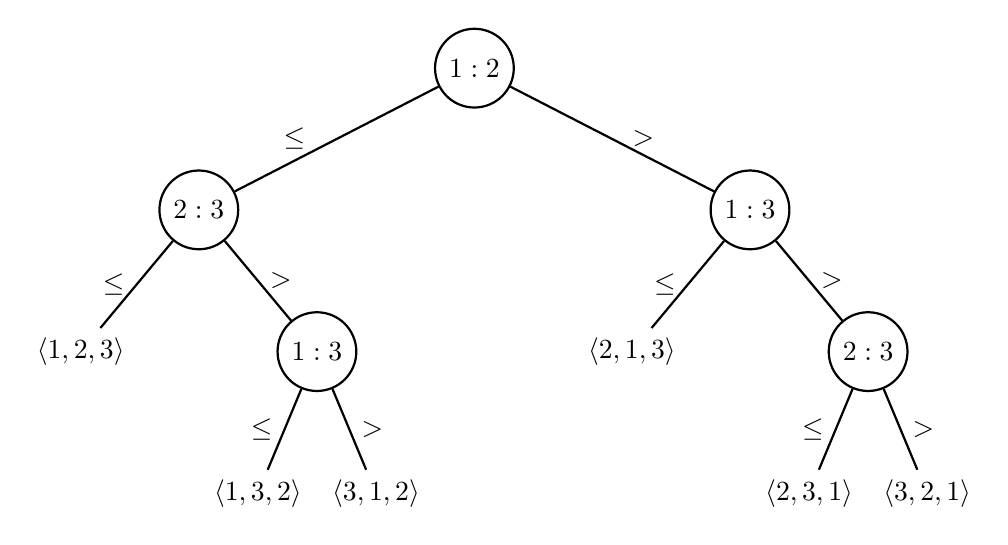
\begin{tikzpicture}[
    level distance=1.8cm,
    level 1/.style={sibling distance=7cm},
    level 2/.style={sibling distance=3cm},
    level 3/.style={sibling distance=1.5cm},
    internal/.style={circle, draw, thick, minimum size=1cm, font=\normalsize},
    leaf/.style={font=\normalsize},
    edge from parent/.style={draw, thick},
    edge label/.style={font=\normalsize, inner sep=2pt}
]

% Root
\node[internal] {$1:2$}
    child {
        node[internal] {$2:3$}
        child {
            node[leaf] {$\langle 1,2,3 \rangle$}
            edge from parent node[left, edge label, xshift=-2pt] {$\le$}
        }
        child {
            node[internal] {$1:3$}
            child {
                node[leaf] {$\langle 1,3,2 \rangle$}
                edge from parent node[left, edge label, xshift=-2pt] {$\le$}
            }
            child {
                node[leaf] {$\langle 3,1,2 \rangle$}
                edge from parent node[right, edge label, xshift=2pt] {$>$}
            }
            edge from parent node[right, edge label, xshift=2pt] {$>$}
        }
        edge from parent node[left, edge label, xshift=-9pt] {$\le$}
    }
    child {
        node[internal] {$1:3$}
        child {
            node[leaf] {$\langle 2,1,3 \rangle$}
            edge from parent node[left, edge label, xshift=-2pt] {$\le$}
        }
        child {
            node[internal] {$2:3$}
            child {
                node[leaf] {$\langle 2,3,1 \rangle$}
                edge from parent node[left, edge label, xshift=-2pt] {$\le$}
            }
            child {
                node[leaf] {$\langle 3,2,1 \rangle$}
                edge from parent node[right, edge label, xshift=2pt] {$>$}
            }
            edge from parent node[right, edge label, xshift=2pt] {$>$}
        }
        edge from parent node[right, edge label, xshift=5pt] {$>$}
    };

\end{tikzpicture}
\caption{A decision tree for a comparison-based sorting algorithm on three distinct elements, inspired by the decision-tree illustration in \emph{Introduction to Algorithms}~\cite{CLRS09}. Each internal node represents a comparison $a_i \le a_j$, and each leaf corresponds to a permutation of the input elements.}
\label{fig:decision-tree-3}
\end{figure}

To reason about all possible executions of a comparison sort, we model the algorithm as a decision tree.
Figure~\ref{fig:decision-tree-3} illustrates this abstraction for a sorting algorithm operating on three distinct elements.

\begin{definition}[Decision Tree]
A \emph{decision tree} for a comparison sort on $n$ elements is a full binary tree with the following properties:
\begin{itemize}
    \item Each internal node is labeled by a comparison $i : j$, representing a test of whether $a_i \le a_j$.
    \item The left child corresponds to the outcome $a_i \le a_j$, and the right child corresponds to $a_i > a_j$.
    \item Each leaf is labeled by a permutation $(\pi(1), \pi(2), \dots, \pi(n))$, indicating the final ordering
    \[
    a_{\pi(1)} \le a_{\pi(2)} \le \cdots \le a_{\pi(n)}.
    \]
\end{itemize}
\end{definition}

An execution of the sorting algorithm on a particular input corresponds to following a single path from the root of the decision tree to a leaf, determined by the outcomes of the comparisons performed.

Crucially, the decision tree captures only the comparisons made by the algorithm. All other aspects of computation—data movement, control flow, and memory access—are ignored. For comparison sorts, this abstraction is sufficient to reason about worst-case running time.

\section{Why There Must Be Many Leaves}

A correct sorting algorithm must be able to handle every possible input ordering.

Since the $n$ input elements are distinct, there are exactly $n!$ possible permutations of the input. Each permutation represents a different total ordering of the elements.

\begin{lemma}
Every correct comparison sort on $n$ distinct elements must have at least $n!$ reachable leaves in its decision tree.
\end{lemma}

\begin{proof}
Each leaf of the decision tree corresponds to a specific ordering of the input elements. For the algorithm to be correct, it must be able to produce the correct sorted order for \emph{every} permutation of the input.

Therefore, for each of the $n!$ permutations, there must exist at least one root-to-leaf path whose sequence of comparisons is consistent with that permutation. In other words, every permutation must appear as a reachable leaf of the decision tree.

Hence, the decision tree must have at least $n!$ reachable leaves.
\end{proof}

This observation is the combinatorial core of the lower bound: sorting requires distinguishing among $n!$ possible cases.

\section{Height of the Decision Tree and Worst-Case Cost}

The running time of a comparison sort is determined by how many comparisons it performs.

\begin{definition}[Decision-Tree Height]
The \emph{height} of a decision tree is the length of the longest root-to-leaf path.
\end{definition}

In the decision-tree model, each internal node corresponds to exactly one comparison. Thus:

\begin{itemize}
    \item The number of comparisons performed on a particular input equals the length of the corresponding root-to-leaf path.
    \item The worst-case number of comparisons equals the height of the decision tree.
\end{itemize}

Therefore, to prove a lower bound on the worst-case running time of comparison sorting, it suffices to prove a lower bound on the height of any decision tree with at least $n!$ leaves.

\section{Deriving the Lower Bound}

We now connect the number of leaves in a decision tree to its height, which directly determines the worst-case number of comparisons made by a sorting algorithm.

\begin{lemma}
A binary tree of height $h$ has at most $2^h$ leaves.
\end{lemma}

\begin{proof}
At each level of the tree, the number of nodes can at most double. Since the root is at level $0$, a tree of height $h$ has at most $2^h$ leaves.
\end{proof}

Recall that any correct comparison-based sorting algorithm must be able to distinguish among all $n!$ permutations of the input, and therefore its decision tree must have at least $n!$ leaves. Combining this requirement with the previous lemma, we obtain
\[
n! \le 2^h.
\]

Taking logarithms (base $2$) of both sides yields
\[
h \ge \log(n!).
\]

To convert this bound into a more familiar asymptotic form, we use a standard approximation for the factorial function.

\begin{lemma}
\[
\log(n!) = \Theta(n \log n).
\]
\end{lemma}

\begin{proof}
Using Stirling's approximation,
\[
n! \approx \sqrt{2\pi n} \left(\frac{n}{e}\right)^n,
\]
and taking logarithms gives
\[
\log(n!) = n \log n - n \log e + O(\log n).
\]
Thus, $\log(n!)$ grows on the order of $n \log n$.
\end{proof}

Substituting this estimate into the height bound completes the argument.

\begin{theorem}
Any comparison-based sorting algorithm on $n$ elements requires $\Omega(n \log n)$ comparisons in the worst case.
\end{theorem}

\begin{proof}
As shown above, the decision tree of any correct comparison sort must have height at least $\log(n!) = \Omega(n \log n)$. Since the height of the decision tree equals the worst-case number of comparisons performed by the algorithm, the result follows.
\end{proof}

\begin{corollary}
Merge sort and heapsort are asymptotically optimal comparison sorts.
\end{corollary}

\begin{proof}
Both algorithms run in $O(n \log n)$ time in the worst case, matching the $\Omega(n \log n)$ lower bound. No comparison sort can asymptotically outperform them.
\end{proof}

\section{Conclusion}

The $\Omega(n \log n)$ lower bound for comparison-based sorting is a foundational result in algorithm analysis. It follows from a simple observation: sorting requires distinguishing among $n!$ possible input orderings, while each comparison provides only limited information.

By modeling comparison-based sorting algorithms as decision trees, this intuition becomes a precise mathematical argument. The result explains why no comparison-based algorithm can asymptotically outperform $O(n \log n)$ sorting.

It is important to note that this lower bound applies only within the comparison model. Algorithms such as counting sort and radix sort achieve linear-time performance by exploiting additional assumptions about the input and therefore do not contradict the bound.

\begin{thebibliography}{CLRS09}
\setlength{\labelsep}{0.8em}

\bibitem[CLRS09]{CLRS09}
T. H. Cormen et al.,
\emph{Introduction to Algorithms}, 3rd ed., MIT Press, 2009.

\bibitem[KT06]{KT06}
J. Kleinberg and \'{E}. Tardos,
\emph{Algorithm Design}, Pearson, 2006.

\bibitem[AHU74]{AHU74}
    A. V. Aho, J. E. Hopcroft, and J. D. Ullman,
    \emph{The Design and Analysis of Computer Algorithms}, Addison-Wesley, 1974.

\end{thebibliography}

\end{document}
